% !TEX TS-program = pdflatex
% !TEX encoding = UTF-8 Unicode

% This is a simple template for a LaTeX document using the "article" class.
% See "book", "report", "letter" for other types of document.

\documentclass[11pt]{article} % use larger type; default would be 10pt

\usepackage{amsmath,amssymb}
\usepackage[utf8]{inputenc} % set input encoding (not needed with XeLaTeX)

%%% Examples of Article customizations
% These packages are optional, depending whether you want the features they provide.
% See the LaTeX Companion or other references for full information.

%%% PAGE 
\usepackage{geometry} % to change the page dimensions
\geometry{letterpaper} % or letterpaper (US) or a5paper or....
% \geometry{margin=2in} % for example, change the margins to 2 inches all round
% \geometry{landscape} % set up the page for landscape
%   read geometry.pdf for detailed page layout information

\usepackage{graphicx} % support the \includegraphics command and options

% \usepackage[parfill]{parskip} % Activate to begin paragraphs with an empty line rather than an indent

%%% PACKAGES
\usepackage{booktabs} % for much better looking tables
\usepackage{array} % for better arrays (eg matrices) in maths
\usepackage{paralist} % very flexible & customisable lists (eg. enumerate/itemize, etc.)
\usepackage{verbatim} % adds environment for commenting out blocks of text & for better verbatim
\usepackage{subfig} % make it possible to include more than one captioned figure/table in a single float
% These packages are all incorporated in the memoir class to one degree or another...

%%% HEADERS & FOOTERS
\usepackage{fancyhdr} % This should be set AFTER setting up the page geometry
\pagestyle{fancy} % options: empty , plain , fancy
\renewcommand{\headrulewidth}{0pt} % customise the layout...
\lhead{}\chead{}\rhead{}
\lfoot{}\cfoot{\thepage}\rfoot{}

%%% SECTION TITLE APPEARANCE
\usepackage{sectsty}
\allsectionsfont{\sffamily\mdseries\upshape} % (See the fntguide.pdf for font help)
% (This matches ConTeXt defaults)

%%% ToC (table of contents) APPEARANCE
\usepackage[nottoc,notlof,notlot]{tocbibind} % Put the bibliography in the ToC
\usepackage[titles,subfigure]{tocloft} % Alter the style of the Table of Contents

\usepackage{xcolor}

\renewcommand{\cftsecfont}{\rmfamily\mdseries\upshape}
\renewcommand{\cftsecpagefont}{\rmfamily\mdseries\upshape} % No bold!

\newcommand{\ns}[1]{\textcolor{red}{#1}}
%%% END Article customizations

%%% The "real" document content comes below...

\title{Consequences of Pauli blocking between paired fermions on Feshbach resonances}
%\author{The Author}
%\date{} % Activate to display a given date or no date (if empty),
         % otherwise the current date is printed 
\input{../newcommand}
\begin{document}
\maketitle

\section{Model system}

We consider a system made of two different fermionic atoms, $\alpha$ and $\beta$.  These fermions can be in two coupled subbands. Let $\alpha^{\dg}_{\vk, \nu}$ and $\beta^{\dg}_{\vk,\nu}$, be the creation operators of fermions $\alpha$ and $\beta$ with momentum $\vk$ in one of their two subbands, $\nu=\pm1$. 

The Hamiltonian f this two-atom system reads as 
\begin{equation}
\mathcal{H}=\mathcal{H}_0+\mathcal{V}
\end{equation}
$\mathcal{H}_0$ is e free fermionic kinetic energy. 	
\begin{equation}
\mathcal{H}_0=\sum_{\nu=\pm1}\sum_{\vk}{(\epsilon_{\mathbf{k}}+\delta^{(\alpha)}_{\nu})\alpha^{\dg}_{\vk, \nu}\alpha^{}_{\vk, \nu}
+(\epsilon_{\mathbf{k}}+\delta^{(\beta)}_{\nu})\beta^{\dg}_{\vk, \nu}\beta^{}_{\vk, \nu}}				
\end{equation}	
where $\epsilon_{\mathbf{k}}=k^2/2m$ if these two atoms are taken with the same mass.  The lowest energy of the two $\alpha$ and $\beta$ subbands are $\eta_{\nu}^{(\alpha)}$ and 	 $\eta_{\nu}^{(\beta)}$ respectively. 

These $(\alpha,\beta)$ fermions are assumed to interact through a BCS-like separable potential having diagonal and non-diagonal processes.  This interaction potential, shown with 1, can be written as 
\begin{equation}\label{eq:V}
\mathcal{V}=-\sum_{\{\nu\}}\sum_{\vk\vk'}w_{\vk}w_{\vk'}V 
\begin{pmatrix}
\nu_{\alpha}^{'}&\nu_{\alpha}^{}\\
\nu_{\beta}^{'}&\nu_{\beta}^{}
\end{pmatrix}
B^{\dg}_{\mathbf{k}^{'},\nu_{\alpha}^{'},\nu_{\beta}^{'}}
B^{}_{\mathbf{k}^{ },\nu_{\alpha}^{},\nu_{\beta}^{}}
\end{equation}
where, in order for $\mathcal{V}$ to be equal  $\mathcal{V}^{\dg}$, the $V 
\left(\begin{smallmatrix}
\nu_{\alpha}^{'}&\nu_{\alpha}^{}\\
\nu_{\beta}^{'}&\nu_{\beta}^{}
\end{smallmatrix}\right)$ prefactor is taken equal to $V 
\left(\begin{smallmatrix}
\nu_{\alpha}^{}&\nu_{\alpha}^{'}\\
\nu_{\beta}^{}&\nu_{\beta}^{'}
\end{smallmatrix}\right)$. 
$w_{\mathbf{k}}$ is a sharp cut-off function taken as identical for all interaction processes for simplicity. This cut-off allows us to get rid of spurious .  The operator   $B^{\dg}_{\mathbf{k}^{ },\nu_{\alpha}^{},\nu_{\beta}^{}}$ creates an $(\alpha,\beta)$ pair with zero total momentm. The fermion $\alpha$ being in the subband $\nu_{\alpha}$ and the fermion $\beta$ in the subband $\nu_{\beta}$.  It reads 
\begin{equation}
B^{\dg}_{\mathbf{k}^{ },\nu_{\alpha}^{},\nu_{\beta}^{}}=a^{\dg}_{\mathbf{k}^{ },\nu_{\alpha}^{}}
b^{\dg}_{-\mathbf{k}^{ },\nu_{\beta}^{}}
\end{equation}
\begin{figure}[htbp]
\begin{center}
\includegraphics[width=0.8\textwidth]{VPair}
\caption{One pair interaction\label{fig:VPair}} 
%\parbox{0.7\textwidth}{\small }

\end{center}
\end{figure}


In order to study the effect of the Puli exclusion principle on paired fermions in coupled subbands, we are going to concentrate on two sets of interaction scatterings.  
\begin{enumerate}
\item The first set deals with pairs made of fermions, $\alpha$ and $\beta$, in different subbands, namely $P^{\dg}_{\vk,1,1}$ and $P^{\dg}_{\vk,-1,-1}$. These fermion pairs will then interact through the diagonal processes of Fig. \ref{fig:intra}, with a scattering called $v_{\eta}$, and through the non-diagonal process of Fig. \ref{fig:inter}, with a transfer scattering called $\tau$.  All the other $V 
\left(\begin{smallmatrix}\nu_{\alpha}^{'}&\nu_{\alpha}^{}\\ \nu_{\beta}^{'}&\nu_{\beta}^{}\end{smallmatrix}\right)$ scatterings are taken equal to zero.  When the number of fermions $\alpha$ and $\beta$ increases, the pairs $(\nu_{\alpha}=1, \nu_{\beta}=1)$ feel each other by Pauli blocking, as well as the pairs $(\nu_{\alpha}=-1, \nu_{\beta}=-1)$.
\begin{figure}[hhtb]
	\centering
	         \subfloat[Diagonal interaction]{\label{fig:intra}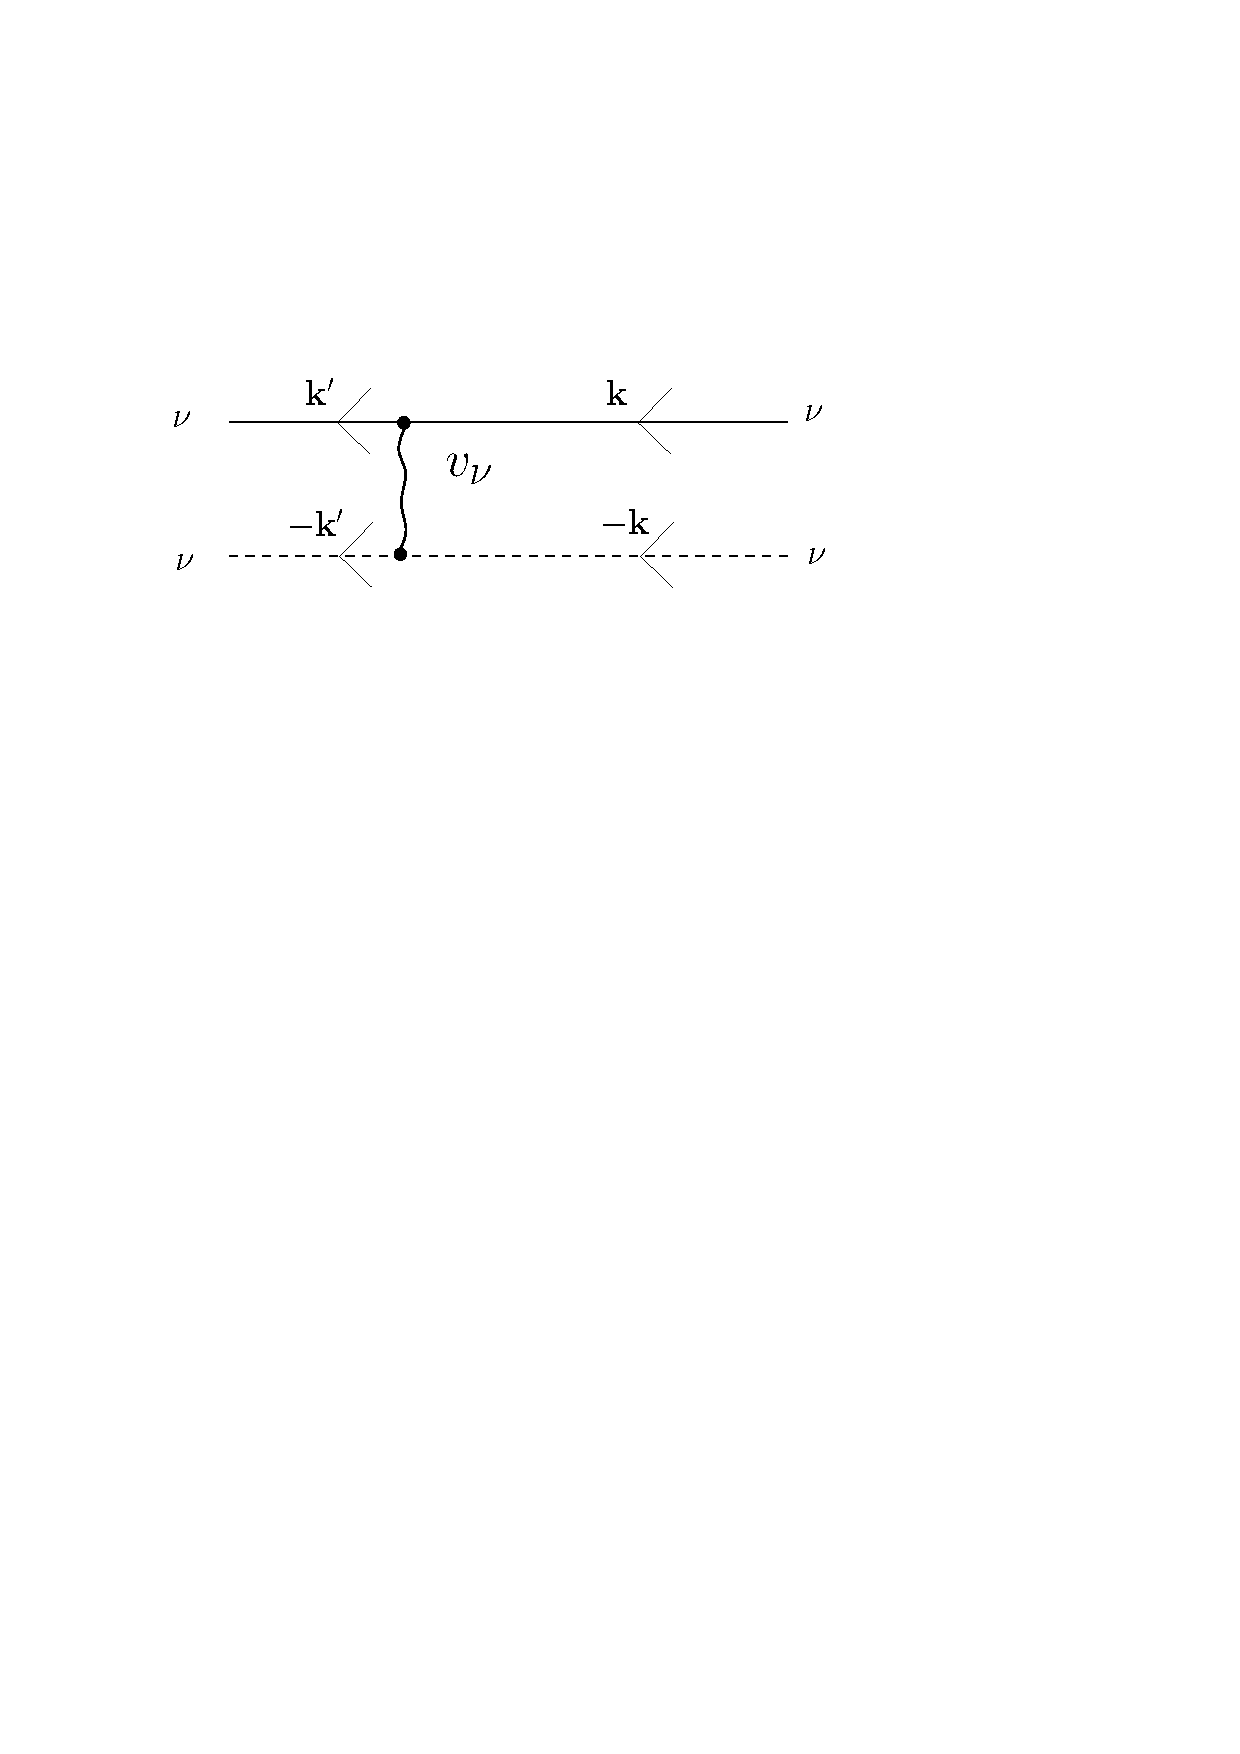
\includegraphics[width=.3\textwidth]{intraBand}}\quad
		\subfloat[Non-diagonal interaction]{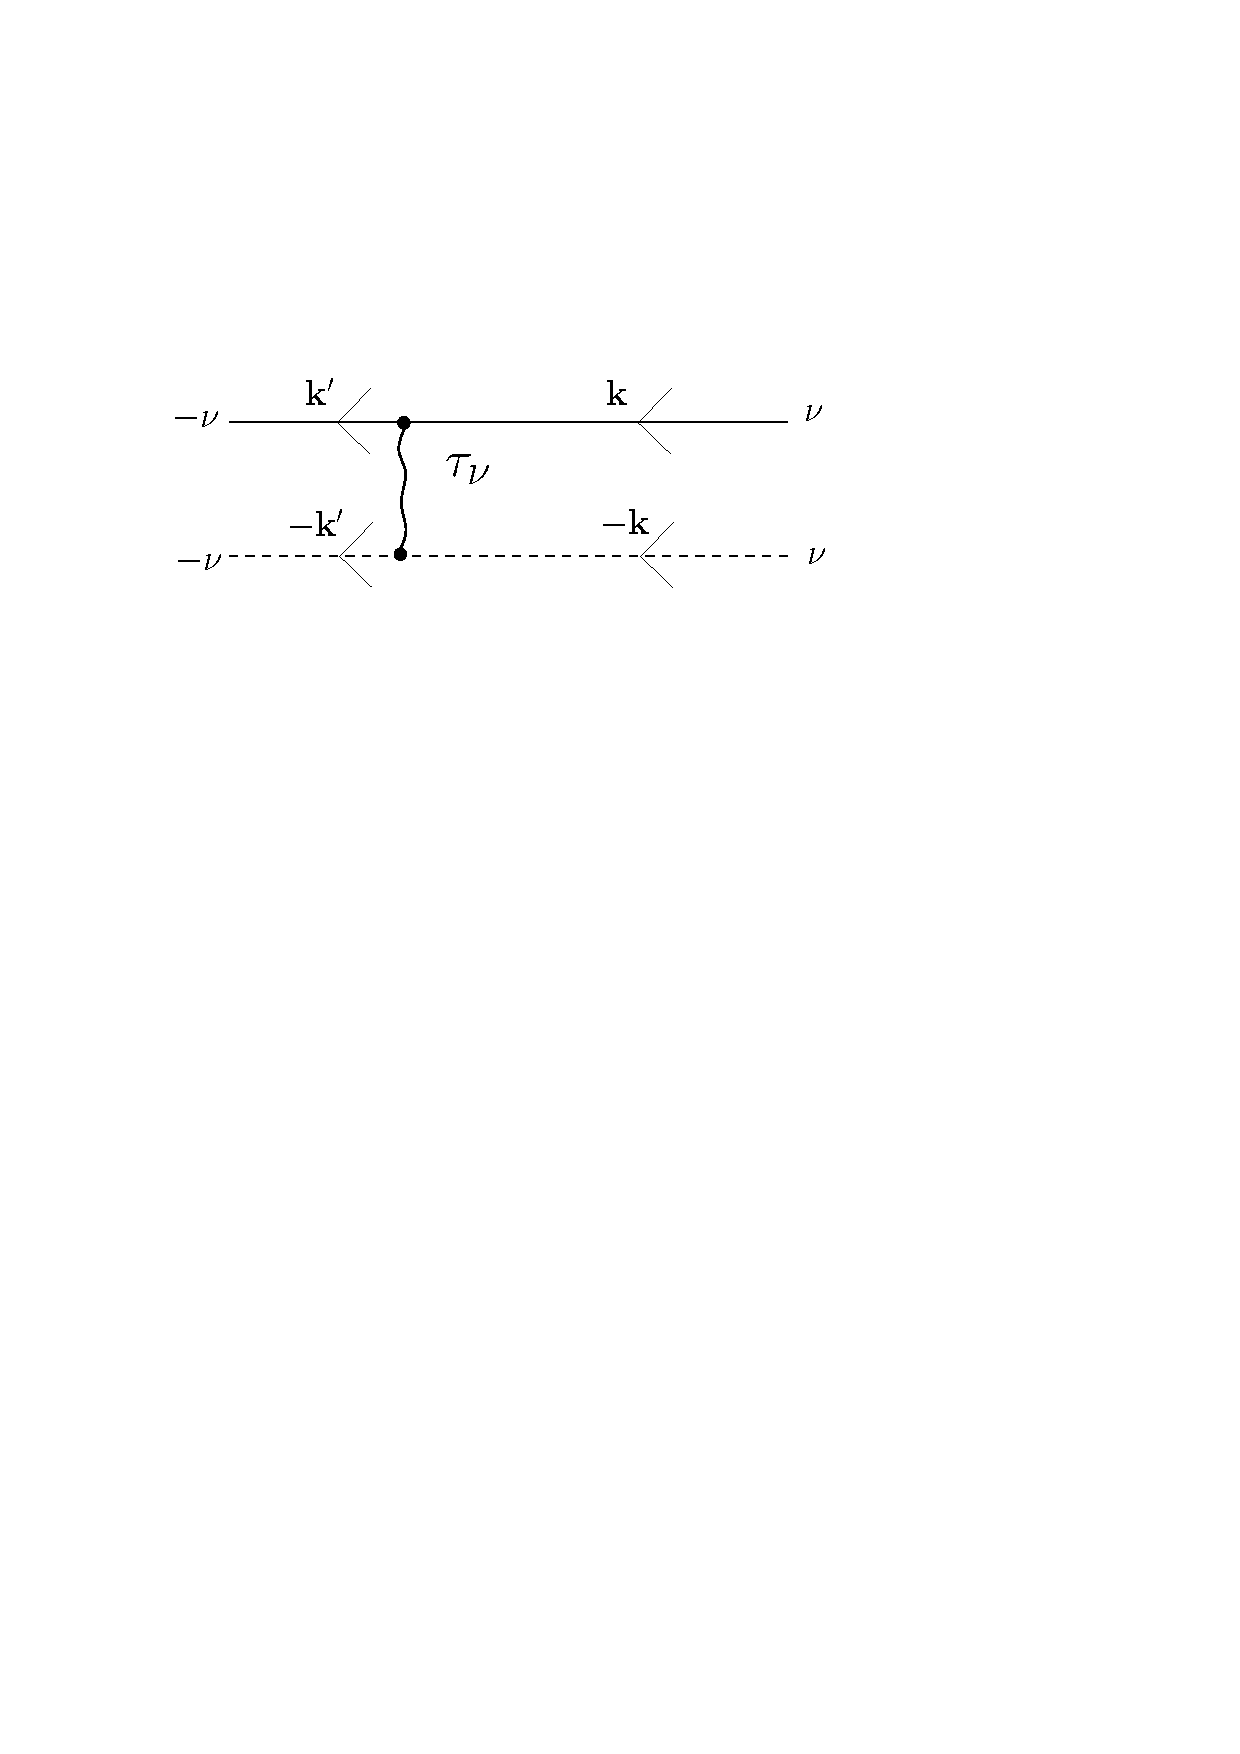
\includegraphics[width=.30\textwidth]{interBand}\label{fig:inter}}
	\caption{Diagonal and non-diagonal subband interaction without shared species}
\end{figure}
\item The second set of interaction potentials deal with pairs sharing a fermion $\alpha$ in subband $1$, namely $B^{\dg}_{\vk,1,1}$ and $B^{\dg}_{\vk,-1,-1}$. These fermion pairs interact through the diagonal processes of Fig. \ref{3intraBand} with a transfer scattering $\tau$, the fermion $\alpha$ now staying in the $\nu=1$ band.  All the other $V 
\left(\begin{smallmatrix}\nu_{\alpha}^{'}&\nu_{\alpha}^{}\\ \nu_{\beta}^{'}&\nu_{\beta}^{}\end{smallmatrix}\right)$ scatterings are taken equal to zero.  In this case, the $(-1)$ states of fermion $\alpha$ stay uncoupled and play no role in the problem.  When the number of fermions $\alpha$ and $\beta$ increases, a $B^{\dg}_{\vk,1,1}$ pair feels not only the other $B^{\dg}_{\vk,1,1}$ pairs by Pauli blocking, but it also feels the $B^{\dg}_{\vk,1,-1}$ pairs because $B^{\dg}_{\vk,1,1}$ and $B^{\dg}_{\vk,1,-1}$ share the same fermion operator $a^{\dg}_{\vk,1}$.
\begin{figure}[hhtb]
	\centering
	         \subfloat[Diagonal interaction]{\label{fig:3intra}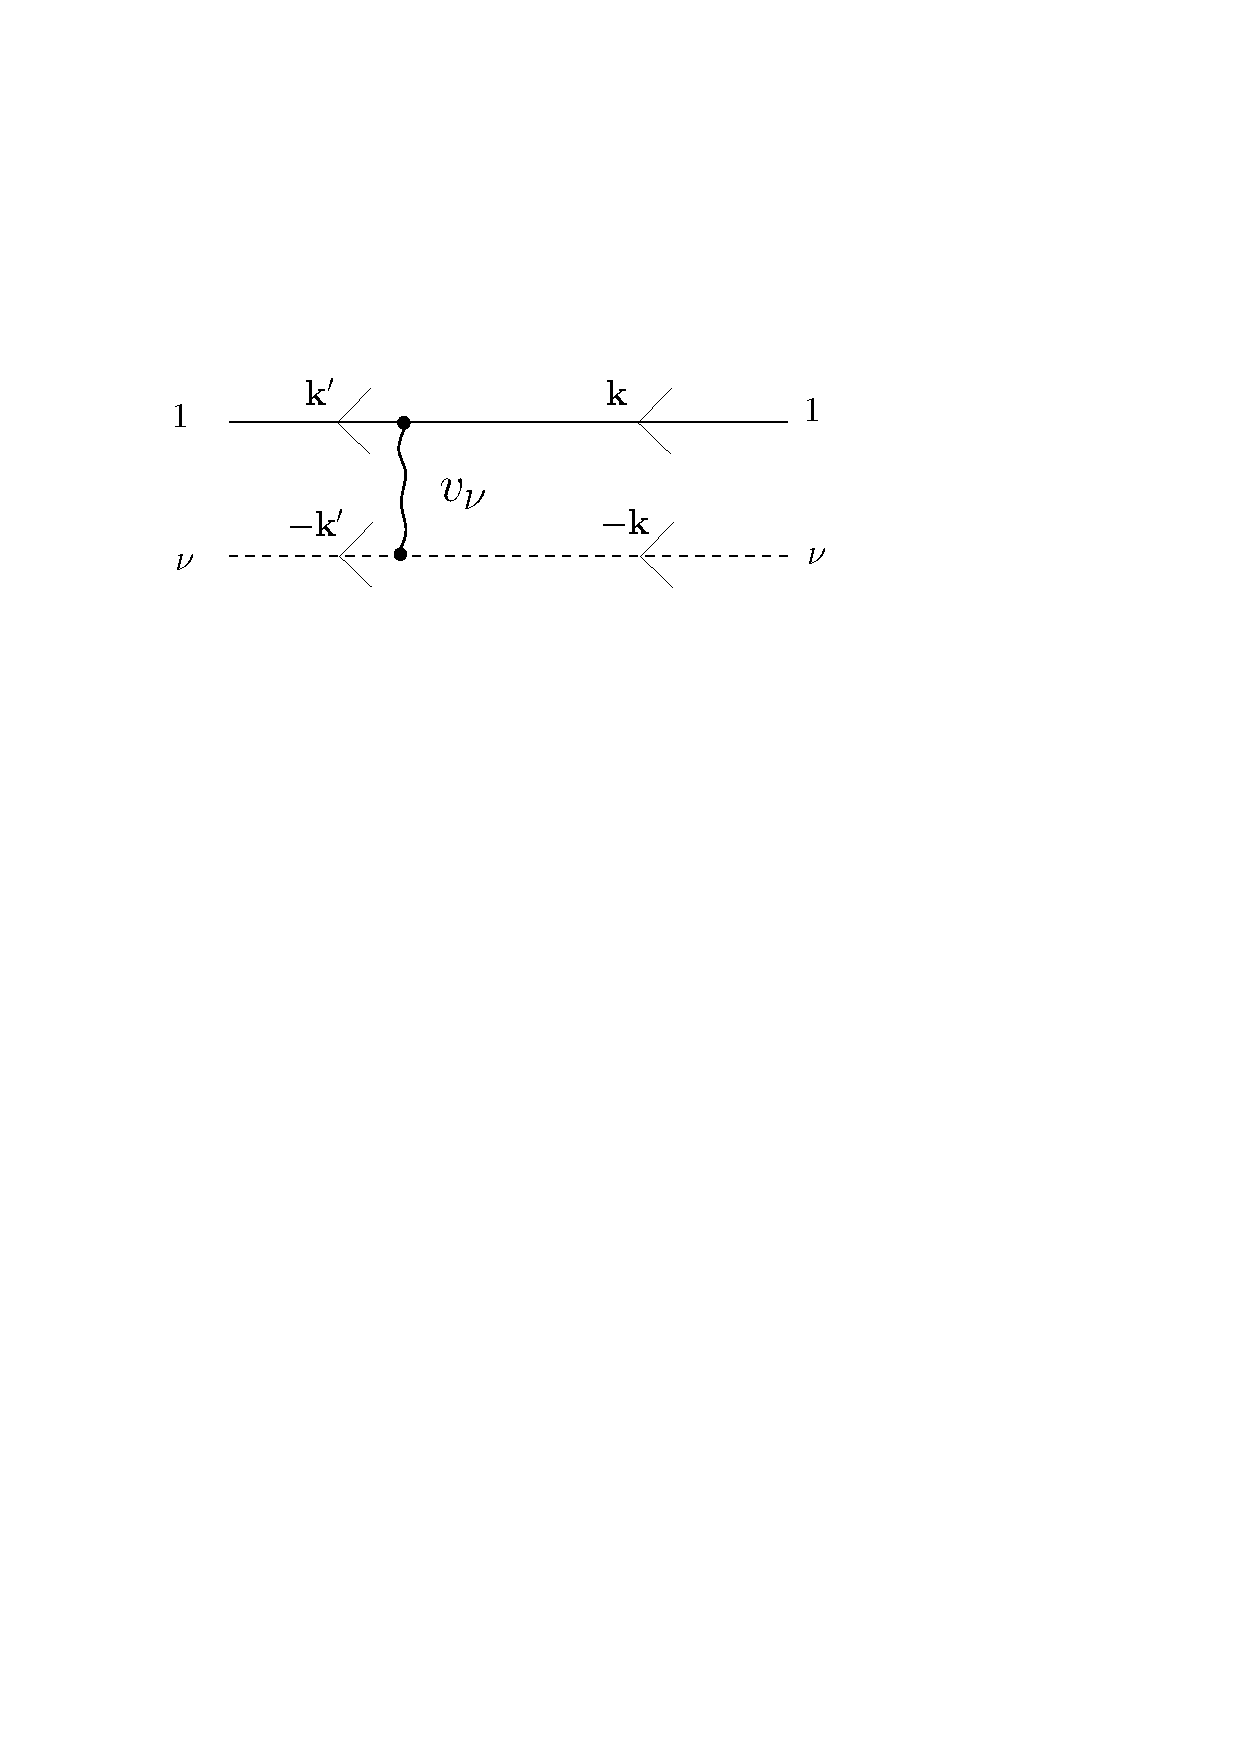
\includegraphics[width=.3\textwidth]{3intraBand}}\quad
		\subfloat[Non-diagonal interaction]{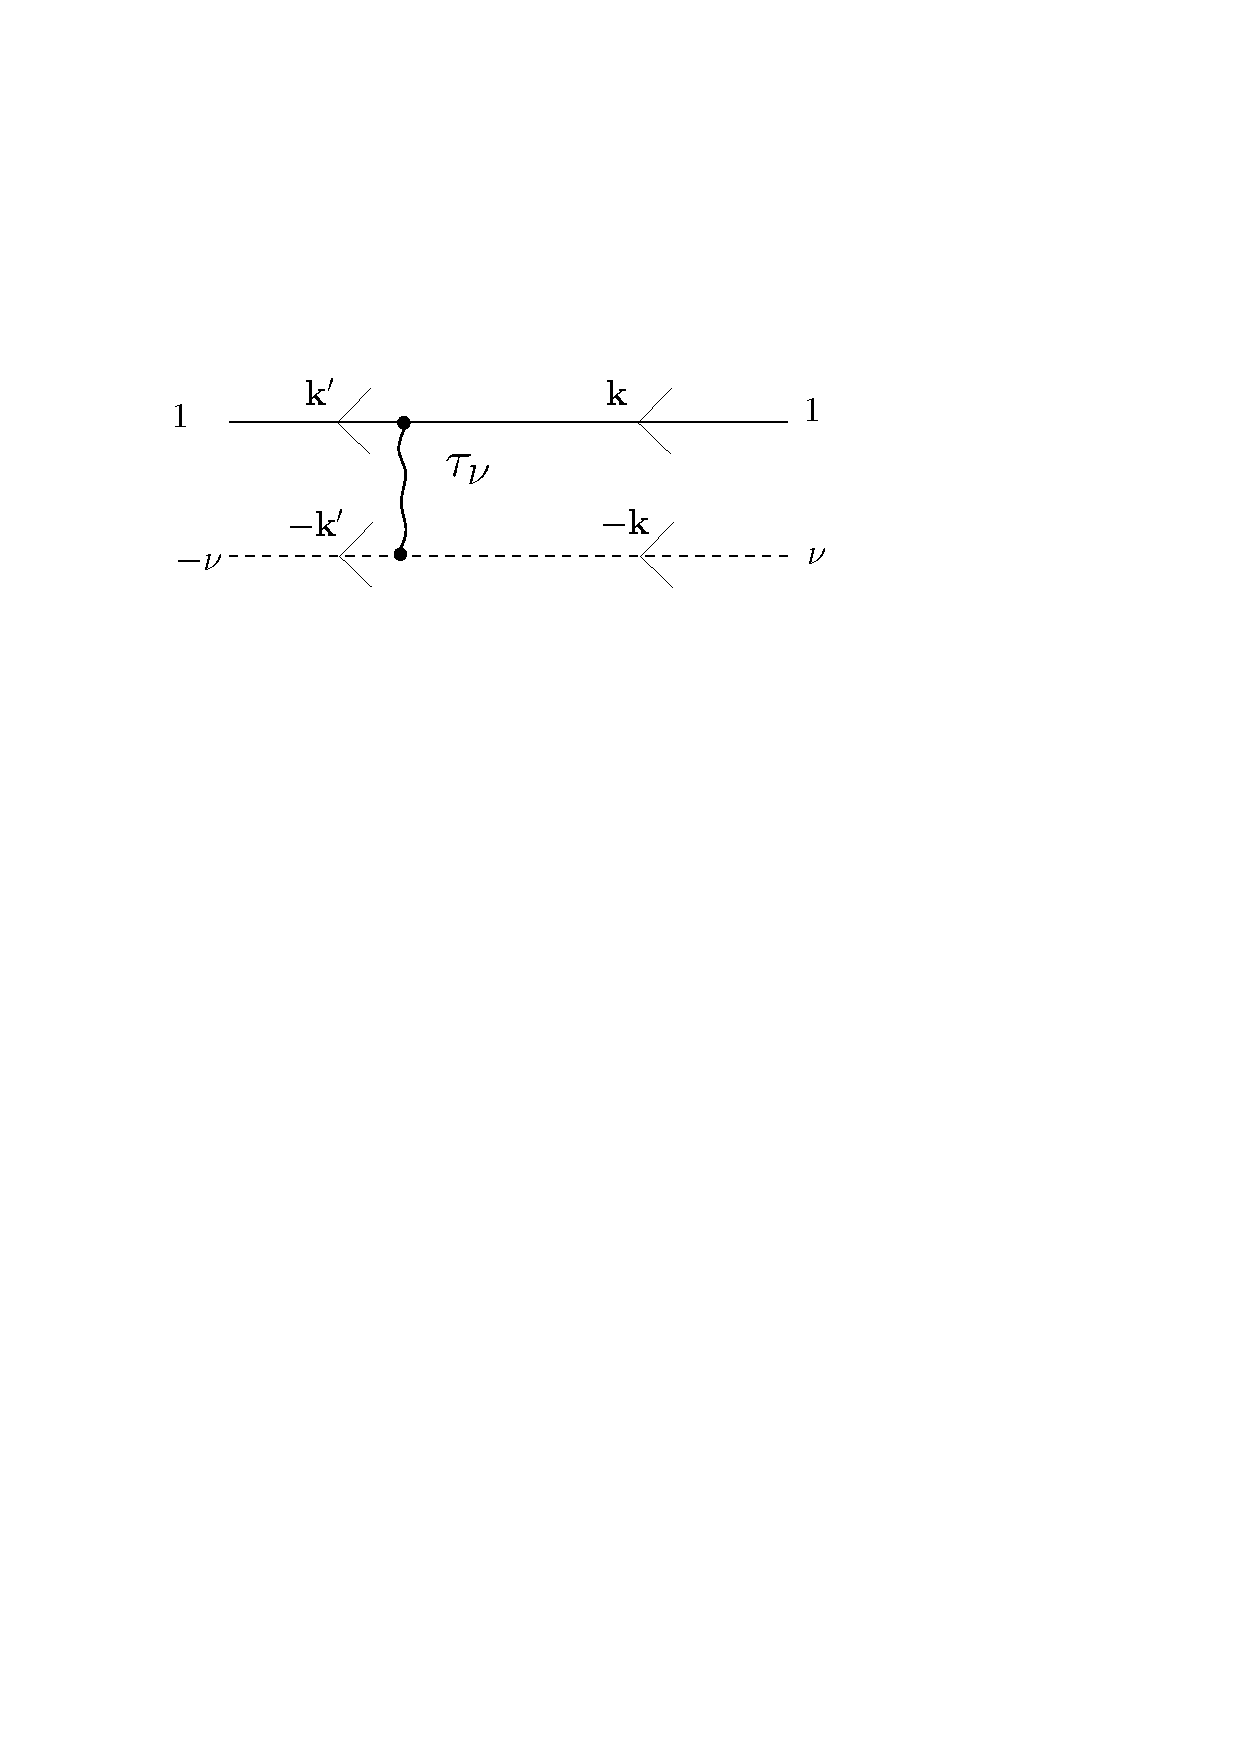
\includegraphics[width=.30\textwidth]{3interBand}\label{fig:3inter}}
	\caption{Diagonal and non-diagonal subband interaction with shared species}
\end{figure}
\end{enumerate}

Comparison between the results obtained within the two sets of interaction scatterings described above will help us to understand the very special role played by the Pauli exclusion principle in composite boson many-body effect, through differentiating Pauli blocking between a given set of pairs $B^{\dg}_{\vk,\eta,\eta}$ and between different sets of pairs $B^{\dg}_{\vk,\eta,\eta}$ and $B^{\dg}_{\vk,\eta,-\eta}$.

Feshbach resonances provide a very unique tool to test this understanding. Indeed, by changing the magnetic field felt by the $(\alpha,\beta)$ atoms, we can change the subband energy differences $\eta^{(\alpha)}=\eta^{(\alpha)}_1-\eta^{(\alpha)}_{-1}$ and  $\eta^{(\beta)}=\eta^{(\beta)}_1-\eta^{(\beta)}_{-1}$ without substantially changing the potential scattering $v_{\eta}$ and $\tau$.  In the absence of subband \ns{transfer}, $\tau=0$, a pair if fermions $(\alpha,\beta)$ in subband $1$ can have a bound state if $v_1$ is large enough.  By changing the magnetic field, the pair energy of this bound state, $\eta^{(\alpha)}_1+\eta^{(\beta)}_{1}-\epsilon_1^*$ when $\epsilon_1^*$ is the bound state binding energy, can cross the energy  $\eta^{(\alpha)}_{-1}+\eta^{(\beta)}_{-1}$ or  $\eta^{(\alpha)}_{1}+\eta^{(\beta)}_{-1}$ of a fermion pair in the $(-1)$ subband, ``open channel'', i.e., when the $v_{-1}$ potential is too small to bind a  $(\alpha,\beta)$ pair. The goal of the present work is to describe this anticrossing in the presence of a finite potential $\tau$.  If we only have one fermion air  $(\alpha,\beta)$, the problem is  rather simple to the single Cooper pair problem and the exact analytical result is easy to extend to finite $\tau$.  The interesting question raised by Pauli blocking between fermion pairs sharing a common fermion, \ns{case} when the number of pairs gets larger than $1$.  The energy of two Cooper pairs with Pauli blocking between them treated exactly has recently been bound in the absence of coupling $\tau$\cite{combescotBCS}.  Its extension to finite $\tau$ to finite $\tau$ \ns{yet} is quite valuable as it indicates the trend induced by the Pauli exclusion principle on the single pair solution.  As already shown in the absence of transfer, $\tau=0$, this trend is of great help to physically understand what the Pauli exclusion really does in the far more complex case of $N$ pairs and more generally along the BEC-BCS crossover in a two channel configuration. 

\section{Commutation relations}
A nice way to handle the Pauli exclusion principle between paired fermions is through a commutation formalism similar to the one we developed for semiconductor excitons\cite{CobosonPhysicsReports}.  Let us first derive a few commutators useful in the present problem. 

For fermion operators $a^{\dg}_{\vk\nu_{\alpha}}$ and $b^{\dg}_{\vk\nu_{\beta}}$ having standard anticommuation relations, we easily get the following commutators
\begin{equation}
[B^{\dg}_{\mathbf{k}^{'},\nu_{\alpha}^{'},\nu_{\beta}^{'}},B^{\dg}_{\mathbf{k}^{ },\nu_{\alpha}^{},\nu_{\beta}^{}}]=0
\end{equation}
\begin{equation}\label{eq:bb}
[B^{}_{\mathbf{k}^{` },\nu_{\alpha}^{'},\nu_{\beta}^{'}},B^{\dg}_{\mathbf{k}^{ },\nu_{\alpha}^{},\nu_{\beta}^{}}]=
	\delta_{\mathbf{k}^{ },\mathbf{k}^{'}}\delta_{\nu_{\alpha}^{},\nu_{\alpha}^{'}}\delta_{\nu_{\beta}^{},\nu_{\beta}^{'}}-
	D^{}_{\mathbf{k}^{' },\nu_{\alpha}^{'},\nu_{\beta}^{'};\,\mathbf{k}^{ },\nu_{\alpha}^{},\nu_{\beta}^{}}
\end{equation}
The operator $D^{}_{\mathbf{k}^{' },\nu_{\alpha}^{'},\nu_{\beta}^{'};\,\mathbf{k}^{ },\nu_{\alpha}^{},\nu_{\beta}^{}}$ is precisely given by
\begin{equation}
D^{}_{\mathbf{k}^{' },\nu_{\alpha}^{'},\nu_{\beta}^{'};\,\mathbf{k}^{ },\nu_{\alpha}^{},\nu_{\beta}^{}}=
	\delta_{\mathbf{k}^{ },\mathbf{k}^{'}}(\delta_{\nu_{\alpha}^{},\nu_{\alpha}^{'}}b^{\dg}_{-\vk\nu_{\beta}}b^{}_{-\vk\nu_{\beta}^{'}}+\delta_{\nu_{\beta}^{},\nu_{\beta}^{'}}a^{\dg}_{\vk\nu_{\alpha}^{}}a^{}_{\vk\nu_{\alpha}^{'}})
\end{equation}
comes from the composite boson nature of fermion pairs.  This operator gives zero when acting on a vacuum while its effect on other paired electrons follows from 

\begin{equation}
\big[D^{}_{\mathbf{k}^{'' },\nu_{\alpha}^{''},\nu_{\beta}^{''};\mathbf{k}^{' },\nu_{\alpha}^{'},\nu_{\beta}^{'}},\,B^{\dg}_{\mathbf{k}^{ },\nu_{\alpha}^{},\nu_{\beta}^{}}\big]=
	\delta_{\mathbf{k}^{ },\mathbf{k}^{'}}\delta_{\mathbf{k}^{'' },\mathbf{k}^{'}}
	\Big(\delta_{\nu_{\alpha}^{''},\nu_{\alpha}^{'}}\delta_{\nu_{\beta}^{''},\nu_{\beta}^{}}B^{\dg}_{\mathbf{k}^{ },\nu_{\alpha}^{},\nu_{\beta}^{'}}+
	\delta_{\nu_{\alpha}^{''},\nu_{\alpha}^{}}\delta_{\nu_{\beta}^{''},\nu_{\beta}^{'}}B^{\dg}_{\mathbf{k}^{ },\nu_{\alpha}^{'},\nu_{\beta}^{}}\Big)
\end{equation}
Using these commutators, it is easy to find the effects o f the potential $\mathcal{V}$ defined in Eq. \ref{eq:V} on paired electrons while the free part $\mathcal{H}_0$ of the Hamiltonian follows from
\begin{equation}\label{eq:h0B}
\big[H_0,\,B^{\dg}_{\mathbf{k}^{ },\nu_{\alpha}^{},\nu_{\beta}^{}}\big]=
	(2\epsilon_{\vk}+\epsilon_{\nu_{\alpha}\nu_{\beta}})B^{\dg}_{\mathbf{k}^{ },\nu_{\alpha}^{},\nu_{\beta}^{}}
\end{equation}
where 
\begin{equation}
\epsilon_{\nu_{\alpha}\nu_{\beta}}=\eta_{\nu_{\alpha}}^{(\alpha)}+\eta_{\nu_{\beta}}^{(\beta)}
\end{equation}
We now use these commutators to calculate the ground state energy of one and two pairs of fermions $\alpha$ and $\beta$ in the two relevant configurations, namely, when this ground state is made of $(B^{\dg}_{\mathbf{k}^{ },1,1}, B^{\dg}_{\mathbf{k}^{ },-1,-1})$ pairs and when it is made of $(B^{\dg}_{\mathbf{k}^{ },1,1}, B^{\dg}_{\mathbf{k}^{ },1,-1})$ pairs. We expect to see some difference when the fact, that these pairs share a common fermion, plays a role through Pauli blocking.  This is going to happen for more than one fermion pairs.  A new Pauli blocking channel then opens \ns{composed} to the one which already exists when the number of composite bosons goes from $1$ to $2$.  For a deep understanding of these two channels, let us first show that one-fermion pair ground state carefully when a transfer between subbands $1$ and $-1$ exists. 

\section{One-pair ground state}
\subsection{pair made of $(B^{\dg}_{\mathbf{k}^{ },1,1}$ and $B^{\dg}_{\mathbf{k}^{ },-1,-1})$}

The relevant part of the interaction potential $\mathcal{V}$ defined in Eq. \ref{eq:V} then reduced to $V+T$. The diagonal part is given by 
\begin{equation}
V=-\sum_{\nu=\pm1}v_{\nu}\sum_{\vk,\vk^{'}}
w_{\vk}w_{\vk'}
B^{\dg}_{\mathbf{k}^{'},\nu,\nu}
B^{}_{\mathbf{k}^{ },\nu,\nu}
\end{equation}
and the \ns{??} part 
\begin{equation}
T=-\tau\sum_{\nu=\pm1}\sum_{\vk,\vk^{'}}
w_{\vk}w_{\vk'}
B^{\dg}_{\mathbf{k}^{'},-\nu,-\nu}
B^{}_{\mathbf{k}^{ },\nu,\nu}
\end{equation}

Using Eq. \ref{eq:h0B}, we find
\begin{equation}
H_0\,B^{\dg}_{\mathbf{k}^{ },\nu,\nu}|0\rangle=
\big[H_0,\,B^{\dg}_{\mathbf{k}^{ },\nu,\nu}\big]|0\rangle=
(2\epsilon_{\vk}+\eta_{\nu}^{(\alpha)}+\eta_{\nu}^{(\beta)})B^{\dg}_{\mathbf{k}^{ },\nu,\nu}|0\rangle
\end{equation}
Eq. \ref{eq:bb} and the fact that the operator $D^{}_{\mathbf{k}^{'' },\nu_{\alpha}^{''},\nu_{\beta}^{''};\mathbf{k}^{' },\nu_{\alpha}^{'},\nu_{\beta}^{'}}$ gives zero on vacuum, allows us to write the diagonal part $V$ acting on one pair as 
\begin{equation}
VB^{\dg}_{\mathbf{k}^{ },\nu,\nu}|0\rangle=-\sum_{\nu^{'}}v_{\nu^{'}}\sum_{\vp^{'}vp^{}}w_{\vp^{'}}w_{\vp}B^{\dg}_{\mathbf{p}^{ },\nu^{'},\nu^{'}}[B^{}_{\mathbf{p}^{ },\nu^{'},\nu^{'}},B^{\dg}_{\mathbf{k}^{ },\nu,\nu}]|0\rangle=-v_{\nu}w_{\vk}\beta^{\dg}_{\nu,\nu}
\end{equation}
where we have set
\begin{equation}
\beta^{\dg}_{\nu,\nu}=\sum_{\vp^{'}}B^{\dg}_{\mathbf{p}^{'},\nu,\nu}
\end{equation}
In the same way, the transient part of the potential gives
\begin{equation}
TB^{\dg}_{\mathbf{k}^{ },\nu,\nu}|0\rangle=-\tau{}w_{\vk}\beta^{\dg}_{-\nu,-\nu}
\end{equation}

We now look for the one-pair expectation of $\mathcal{H}_0+V+T$ as 
\begin{equation}\label{eq:Psi1}
|\Psi_1\rangle=\sum_{\nu=\pm1}\sum_{\vk}\phi_{\vk,\nu}B^{\dg}_{\mathbf{k}^{ },\nu,\nu}|0\rangle
\end{equation}
The above equations allow us to write the Schr\"odinger equation for one-pair $0=(\mathcal{H}_0+V+T)|\Psi_1\rangle$ as 
\begin{equation}
\begin{split}
0=&\sum_{\nu\vk}(2\epsilon_{\vk}+\eta_{\nu_{\alpha}}^{(\alpha)}+\eta_{\nu_{\beta}}^{(\beta)}-E_1)\phi_{\vk\nu}B^{\dg}_{\mathbf{k}^{ },\nu,\nu}\\
&-\sum_{\nu\vk}w_{\vk}\phi_{\vk,\nu}v_{\nu}\sum_{\vp}w_{\vp}B^{\dg}_{\mathbf{p}^{ },\nu,\nu}
 -\tau\sum_{\nu\vk}w_{\vk}\phi_{\vk,\nu}\sum_{\vp}w_{\vp}B^{\dg}_{\mathbf{p}^{ },-\nu,-\nu}
\end{split}
\end{equation}
By changing $\nu$ to $-\nu$ in the last term, we can rewrite this equation in a compact form as 
\begin{equation}\label{eq:schOne}
\begin{split}
0=&\sum_{\nu\vk}B^{\dg}_{\mathbf{k}^{ },\nu,\nu}\Big\{(2\epsilon_{\vk}+\eta_{\nu_{\alpha}}^{(\alpha)}+\eta_{\nu_{\beta}}^{(\beta)}-E_1)\phi_{\vk\nu}\\
&\quad-w_{\vk}v_{\nu}\sum_{\vp}w_{\vp}\phi_{\vp,\nu}-\tau{}w_{\vk}\sum_{\vp}w_{\vp}\phi_{\vp,-\nu}\Big\}|0\rangle
\end{split}
\end{equation}
This equation imposes the prefactor to be zero. 

(i) For $v_{\nu}=0=\tau$, the solution is $2\epsilon_{\vk}+\eta_{\nu_{\alpha}}^{(\alpha)}+\eta_{\nu_{\beta}}^{(\beta)}=E_1$, i.e. $\phi_{\vk^{'}\nu}=0$ for $\vk^{'}\neq\vk$ while $\phi_{\vk^{'}\nu}$ can differ from zero for  $\vk^{'}\neq\vk$. This result just corresponds to free fermion pairs in two uncoupled subbands, as expected. 

For $v_{\nu}$ or $\tau$ different from zero, the solution of Eq. \ref{eq:schOne} reads
\begin{equation}\label{eq:phi}
\phi_{\vk^{}\nu}=\Big(v_{\nu}\sum_{\vp}w_{\vp}\phi_{\vp,\nu}+\tau{}\sum_{\vp}w_{\vp}\phi_{\vp,-\nu}\Big)
\frac{w_{\vk}}{2\epsilon_{\vk}+\eta_{\nu_{\alpha}}^{(\alpha)}+\eta_{\nu_{\beta}}^{(\beta)}-E_1}
\end{equation}
To get the equation fullfilled by the energy, we multiply the above equation by $w_{\vk}$ and we sum over $\vk$.  This gives 
\begin{equation}\label{eq:phiS}
\sum_{\vk}w_{\vk}\phi_{\vk^{}\nu}=\Big(v_{\nu}\sum_{\vp}w_{\vp}\phi_{\vp,\nu}+\tau{}\sum_{\vp}w_{\vp}\phi_{\vp,-\nu}\Big)
S(E_1-\eta_{\nu_{\alpha}}^{(\alpha)}-\eta_{\nu_{\beta}}^{(\beta)})
\end{equation}
where we have 
\begin{equation}\label{eq:Sdef}
S(E)=\sum_{\vk}\frac{w_{\vk}}{2\epsilon_{\vk}-E}
\end{equation}

This gives two homogeneous equations for $\sum_{\vk}w_{\vk}\phi_{\vk\nu}$ with $\nu=\pm1$. They read
\begin{equation}\label{eq:tauEq}
[1-v_{\nu}S(E_1-\eta_{\nu_{\alpha}}^{(\alpha)}-\eta_{\nu_{\beta}}^{(\beta)})]\sum_{\vk}w_{\vk}\phi_{\vk^{}\nu}
=\tau{}S(E_1-\eta_{\nu_{\alpha}}^{(\alpha)}-\eta_{\nu_{\beta}}^{(\beta)})\sum_{\vk}w_{\vk}\phi_{\vk^{}-\nu}
\end{equation}
These equations have a non-zero solution \ns{found} that their determent is equal to zero.  This gives the one-pair eigenstate through a algebraic  equation which reads as 
\begin{multline}
[1-v_{1}S(E_1-\eta_{1}^{(\alpha)}-\eta_{1}^{(\beta)})][1-v_{-1}S(E_1-\eta_{-1}^{(\alpha)}-\eta_{-1}^{(\beta)})]\\
=\tau^2S(E_1-\eta_{1}^{(\alpha)}-\eta_{1}^{(\beta)})S(E_1-\eta_{-1}^{(\alpha)}-\eta_{-1}^{(\beta)})
\end{multline}
Using Eq. \ref{eq:phi}, we get the one-pair eigenstate given in Eq. \ref{eq:Psi1} as
\begin{equation}
|\Psi_1\rangle=\sum_{\nu=\pm1}\Big(v_{\nu}\sum_{\vp}w_{\vp}\phi_{\vp,\nu}+\tau{}\sum_{\vp}w_{\vp}\phi_{\vp,-\nu}\Big)B^{\dg}_{\nu,\nu}(E_{1})|0\rangle
\end{equation}
where $B^{\dg}_{\nu,\nu}(E_{1})|0\rangle=\sum_{\vk}\frac{w_{\vk}}{2\epsilon_{\vk}+\eta_{\nu_{\alpha}}^{(\alpha)}+\eta_{\nu_{\beta}}^{(\beta)}-E_1}\beta^{\dg}_{\nu,\nu}|0\rangle$ by Cooper, namely Eq. \ref{eq:phiS} allows us to rewrite this equation as 
\begin{equation}
|\Psi_1\rangle=\sum_{\nu=\pm1}\frac{\sum_{\vp}w_{\vp}\phi_{\vp\nu}}{S(E_1-\eta_{\nu_{}}^{(\alpha)}-\eta_{\nu_{}}^{(\beta)})}B^{\dg}_{\nu,\nu}(E_{1})|0\rangle
\end{equation}
It is actually possible to transform this symmetrical expression in $\nu=\pm1$ in order to have the transfer coupling $\tau$ appearing \ns{effectively} in $|\Psi_1\rangle$.  To do it, we rewrite the $\sum_{\vp}w_{\vp}\phi_{\vp\nu}$ sum according to Eq. \ref{eq:tauEq} taken for $\nu=-1$.  We then first write an {irrelevant} prefector $\frac{\sum_{\vp}w_{\vp}\phi_{\vp\nu}}{S(E_1-\eta_{\nu_{}}^{(\alpha)}-\eta_{\nu_{}}^{(\beta)})}$ that $|\Psi_1\rangle$ also reads
\begin{equation}\label{eq:Psi1B}
|\Psi_1\rangle=B^{\dg}_{1,1}(E_{1})|0\rangle+X_{1,-1}B^{\dg}_{-1,-1}(E_{1})|0\rangle
\end{equation}
$X_{1,-1}$ the subband mixing introduced by the potential transfer $\tau$.  It precisely reads
\begin{equation}
X_{1,-1}=\frac{\tau{}S(E_1-\eta_{1}^{(\alpha)}-\eta_{1}^{(\beta)})}{1-v_{\nu}S(E_1-\eta_{-1}^{(\alpha)}-\eta_{-1}^{(\beta)})}
\end{equation}
Eqs. (\ref{eq:tauEq}, \ref{eq:Psi1B}) readily shows that, as expected, the one-pair eigenstates reduces, in the absence of transfer $\tau=0$, to the one-pair eigenstate obtained by Cooper, the pairs being made of fermions $\alpha$ and $\beta$ which either belong to the subbands $1$ with energy $\eta^{(\alpha)}_{1}+\eta^{(\beta}_{1}$ or to the subband $-1$ with energy $\eta^{(\alpha)}_{-1}+\eta^{(\beta}_{-1}$.  For finite transfer $\tau$, the two independent pair solutions which are moreover taken for slightly different energy $E_{1}$ if $\tau$ is small. 

\subsection{Pair made of $P^{\dg}_{\vk,1,1}$ and $P^{\dg}_{\vk,1,-1}$}
We now consider $(\alpha,\beta)$ pairs sharing their fermion $\alpha$, this fermion being in the $\nu=1$ subband only.  The relevant part of the interaction potential $\mathcal{V}$ in Eq. \ref{eq:V} reduces to $V+T$ with a diagonal part now given by  
\begin{equation}
V=-\sum_{\nu=\pm1}v_{\nu}\sum_{\vk,\vk^{'}}
w_{\vk}w_{\vk'}
B^{\dg}_{\mathbf{k}^{'},1,\gamma}
B^{}_{\mathbf{k}^{ },1,\nu}
\end{equation}
and a transfer part given by 
\begin{equation}
T=-\tau\sum_{\nu=\pm1}\sum_{\vk,\vk^{'}}
w_{\vk}w_{\vk'}
B^{\dg}_{\mathbf{k}^{'},1,-\nu}
B^{}_{\mathbf{k}^{ },1,\nu}
\end{equation}
Calculations to derive the single pair eigenstates made of $B^{\dg}_{\mathbf{k}^{'},1,-\nu}$ and $B^{\dg}_{\mathbf{k}^{'},-1,\nu}$ pairs is just the same as the one we did for eigenstates made of $B^{\dg}_{\mathbf{k}^{'},\nu,\nu}$ and $B^{\dg}_{\mathbf{k}^{'},-\nu,-\nu}$ pairs, except that, in Eqs. (\ref{eq:tauEq} \ref{eq:Psi1B}), the fermion $\alpha$ energy $\eta^{(\alpha)}_{\nu}$ is always equal to   $\eta^{(\alpha)}_1$.  The fact that the $B^{\dg}_{\mathbf{k}^{'},1,-\nu}$ and $B^{\dg}_{\mathbf{k}^{'},-1,\nu}$ pairs share a common fermion $\alpha$ is going to be of importance when Pauli blocking enters into the problem, i.e., when we will consider more than one $(\alpha,\beta)$ pair.  

\subsection{Study of $S(E)$}
As seen from the above equations, the one-pair eigenstates are ruled by $S(E)$ defined in Eq. \ref{eq:Sdef}. 

For $3D$ problem with no frozen core, i.e., $w_{\vk}=1$ for $0<\epsilon_{\vk}<\Omega$ and a density of state in $\sqrt{\epsilon_{\vk}}$, we can write $S(E)$ for $E=0$ as 
\begin{equation}
S(E=0)\approx\int_0^{\Omega}\rho(\Omega)\frac{\sqrt{\epsilon/\Omega}}{2\epsilon}d\epsilon
=\frac{\rho(\Omega)}{2}\int_0^1\frac{\sqrt{u}du}{u}=\rho(\Omega)\equiv\rho
\end{equation}
while for finite negative $E$, we find
\begin{equation}
S(E<0)\approx\frac{\rho}{2}\int_0^1\frac{\sqrt{u}du}{u-E/2\Omega}
=\rho\Big(1+\frac{E}{2\Omega}\int_0^1\frac{dx}{x^2-E/2\Omega}\Big)
\end{equation}
which reduces to 
\begin{equation}\label{eq:seNeg}
S(E<0)=\rho\Big(1-\sqrt{\frac{-E}{2\Omega}}\text{Arctg}\sqrt{\frac{2\Omega}{-E}}\Big)
\end{equation}
We can check that $S(E\to0_{-})$ is equal to $\rho$ and $\text{Arctg}(\infty)=\Omega/2$.  Note that for finite positive $E$, we cannot replace the discrete sum over $\vk$ by an integral due to possible divergences for $\epsilon_{\vk}=E$, so that Eq. \ref{eq:seNeg} is not valid anymore.  this actually is unimportant since we are interested in bound states, i.e., negative $E$.

By noting that $1-\sqrt{x}\text{Arctg}(1/\sqrt{x})$ behaves as $1-\pi\sqrt{x}/2$ when $x\to0$ and $1/3x$ when $x\to\infty$, we get 
\begin{gather}
S(E\to0_{-})\approx1-\frac{\pi}{2}\sqrt{\frac{-E}{2\Omega}}\\
S(E\to-\infty)\approx\frac{2\Omega}{-3E}
\end{gather}
$S(E)$ in $3D$ is shown in Fig. (\ref{fig:S3d})
\begin{figure}[hhtb]
	\centering
	         \subfloat{\label{fig:S3d}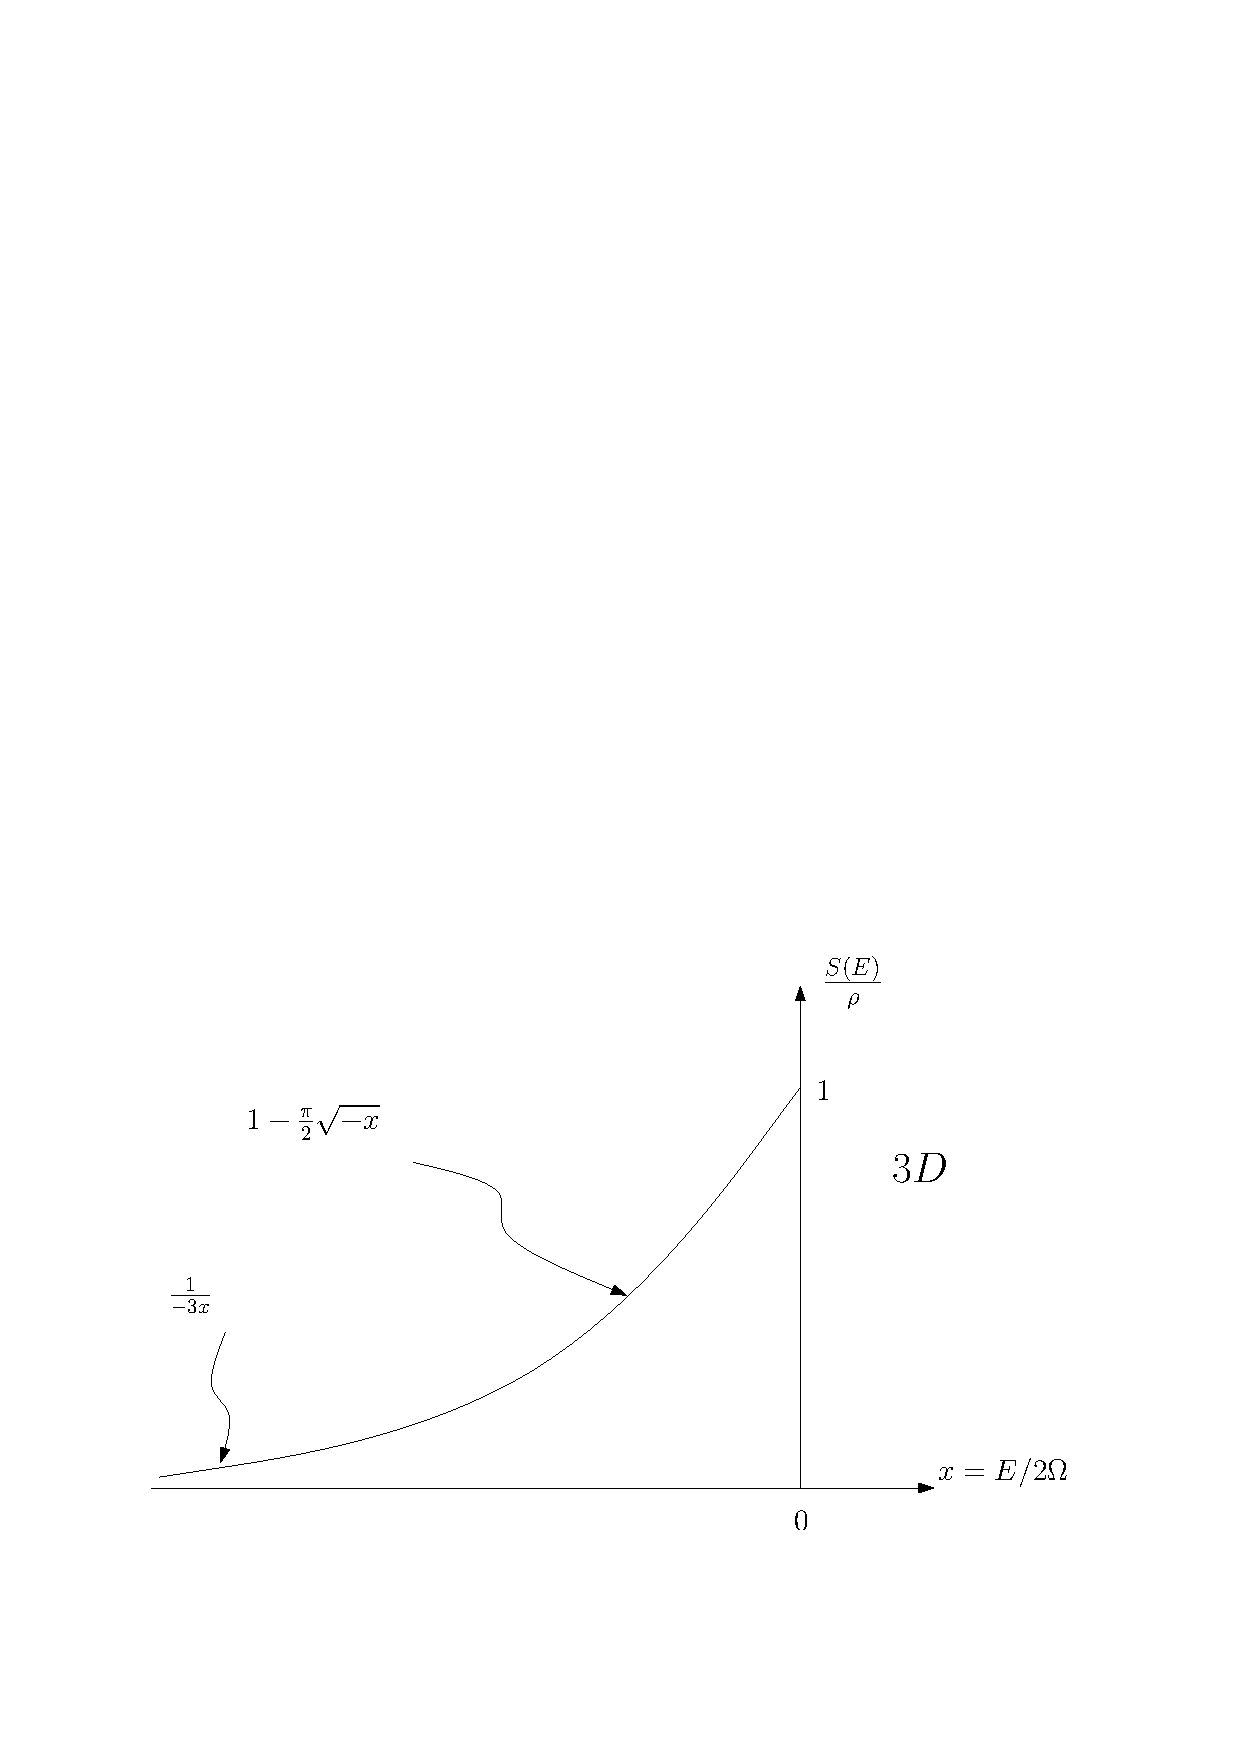
\includegraphics[width=.4\textwidth]{s3d}}\quad
		\subfloat{\label{fig:S2d}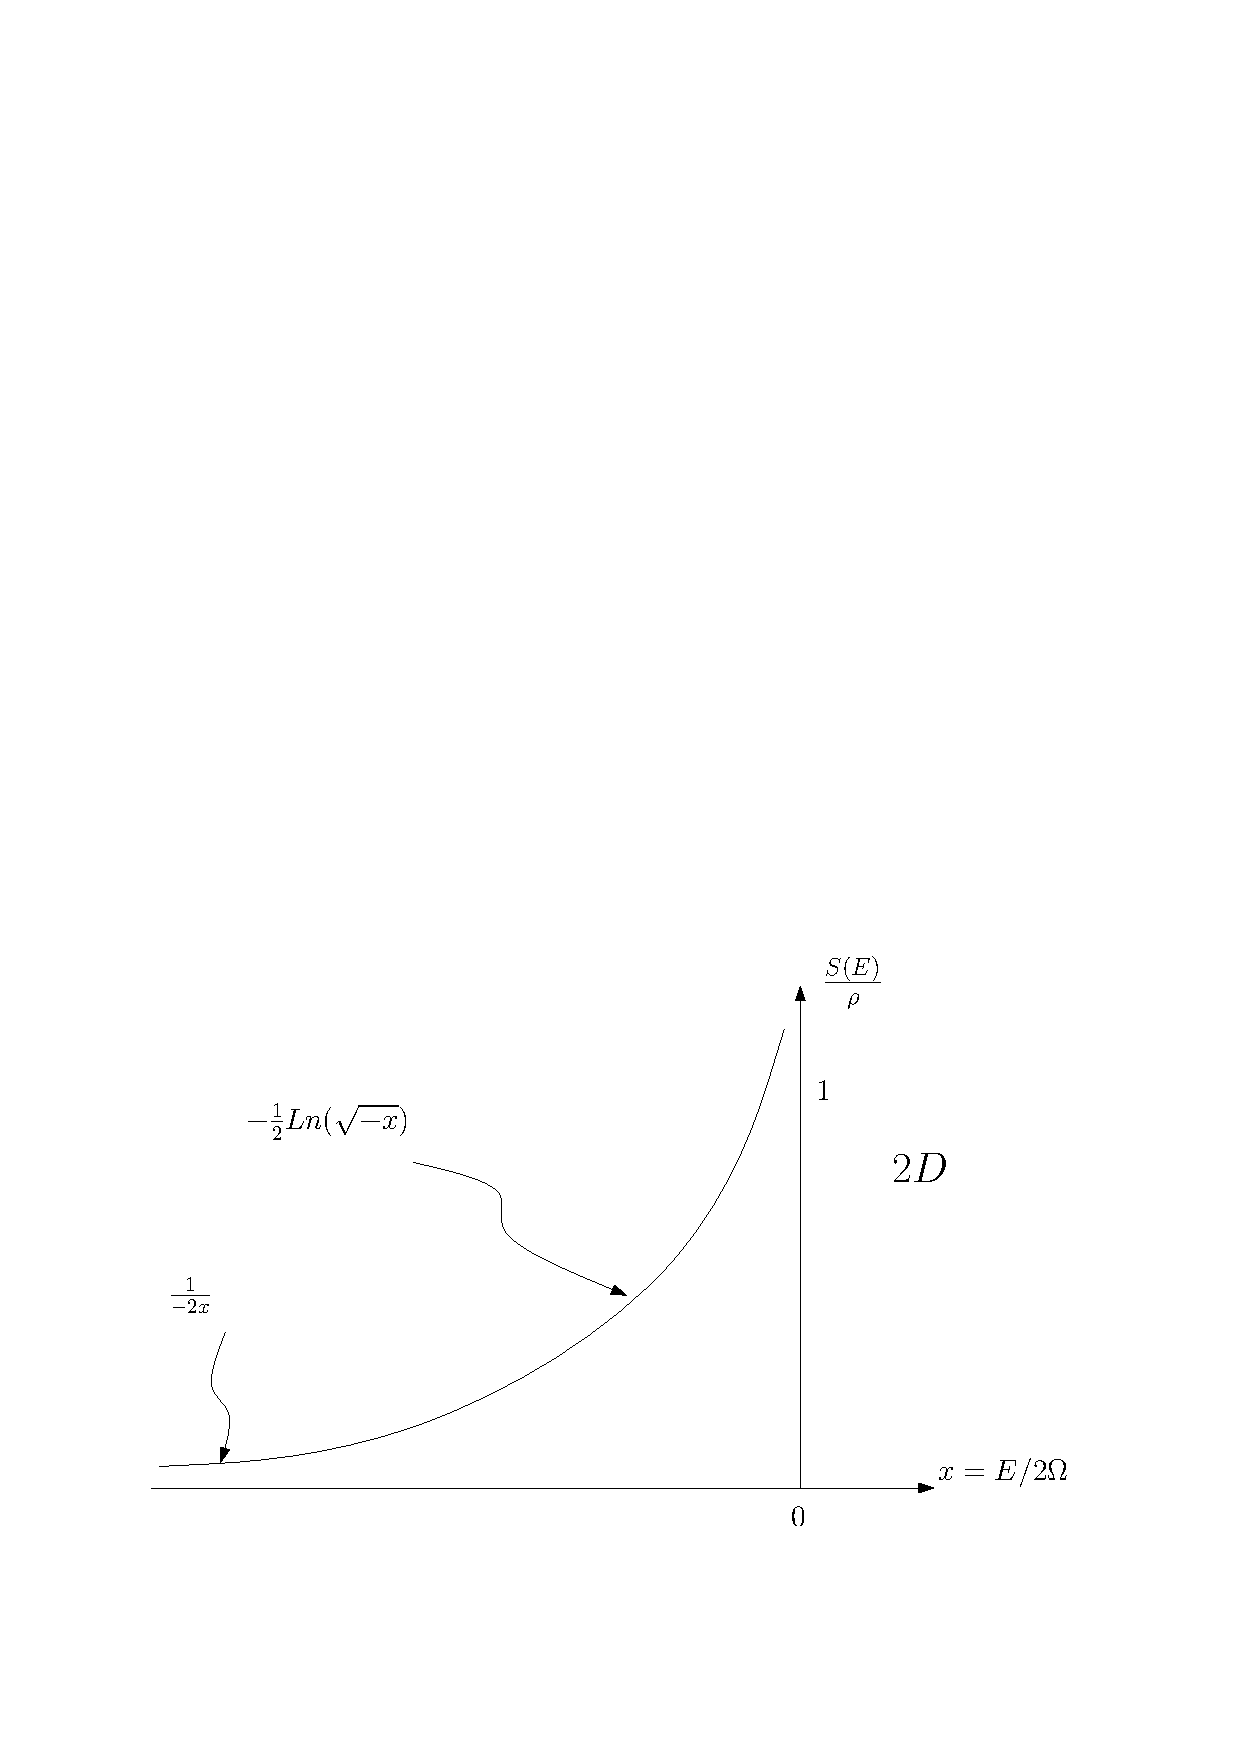
\includegraphics[width=.40\textwidth]{s2d}}\quad
		\caption{$S(E)$ function in $3D$ and $2D$\label{fig:narrowFR}}
\end{figure}
In $2D$ system with no frozen core, we do have since the density of states in the independent of the energy
\begin{equation}
S(E<0)=\int_{0}^{\Omega}\rho\frac{d\epsilon}{2\epsilon-E}=\frac{\rho}{2}\text{Ln}\frac{2\Omega-E}{-E}
\end{equation}
which is again valid in negative $E$ only, due to the replacement of the discrete sum over $\vk$ by an integral and the possible divergences at $\epsilon_{\vk}=E$ for positive $E$. 

The $S(E)$ curves for $3D$ and $2D$ systems are rather similar except that $S(E)$ diverges as $-1/2\text{Ln}(-E/2\Omega)$ when $E$ approaches $0_{-}$ in $2D$ while it stays finite in $3D$.  As a direct consequence, a bound state always exists for a single pair in $2D$, no matter how weak the attractive potential is, while a potential larger than a threshold is necessary in $3D$.

\subsection{Analysis of the one-pair energy}
The one-pair energy follows from 
\begin{equation}\label{eq:ssEq}
[1-v_{1}S(E_1-\epsilon_{1})][1-v_{-1}S(E_1-\epsilon_{-1})]
=\tau^2S(E_1-\epsilon_{1})S(E_1-\epsilon_{-1})
\end{equation}
in which we have set $\epsilon_{-1}=\eta_{-1}^{(\alpha)}+\eta_{-1}^{(\beta)}$ for pairs made of $(B^{\dg}_{\mathbf{k}^{},1,1},B^{\dg}_{\mathbf{k}^{},-1,-1})$ and $\epsilon_{-1}=\eta_{1}^{(\alpha)}+\eta_{-1}^{(\beta)}$ for pairs made of $(B^{\dg}_{\mathbf{k}^{},1,1},B^{\dg}_{\mathbf{k}^{},1,-1})$.

\subsubsection{In the absence of transfer $\tau=0$}
The two types of pairs are then \ns{unrelated}. Pairs in the subband $(\nu_{\alpha}=1,\nu_{\beta}=1)$ have a bound state founded that $1-v_{1}S(E_1-\eta_{1})=0$ has a solution for $E<\epsilon_{1}$.  This always happen in $2D$, no matter how weak $v_{1}$ is since $S(E)$ diverges when $E$ approach $0$. By contrast, $v_{1}$ must be large than a threshold for a bound state to exact in $3D$.  This threshold potential is given by 
\begin{equation}
0=1-v_{\text{th}}S(0)=1-v_{\text{th}}\rho
\end{equation}
Another threshold potential is of physical interest. It corresponds to the bound state for the subbands $(1,1)$ crossing the energy of a free pair with energy $\epsilon_{-1}$ in the subbands $(-1,-1)$ or $(1,-1)$.  This potential threshold $v^{*}$ corresponds to
\begin{equation}
0=1-v^{*}S(\epsilon_{-1}-\epsilon_{1})
\end{equation}

So we end in $3D$ with
\begin{itemize}
\item no bound state below $\epsilon_{1}$ for $0<v_{1}<v_{\text{th}}$;
\item a bound state below $\epsilon_{1}$ for $E$, such that $1-v^{*}S(\epsilon_{-1}-\epsilon_{1})=0$, this bound state being above $\epsilon_{-1}$ for $v_{\text{th}}<v<v^{{*}}$ and below $\epsilon_{-1}$ for $v^{*}<v_{1}$ (see Fig \ref{fig:sDetail})
\end{itemize}
\begin{figure}[htb]
	\centering
	       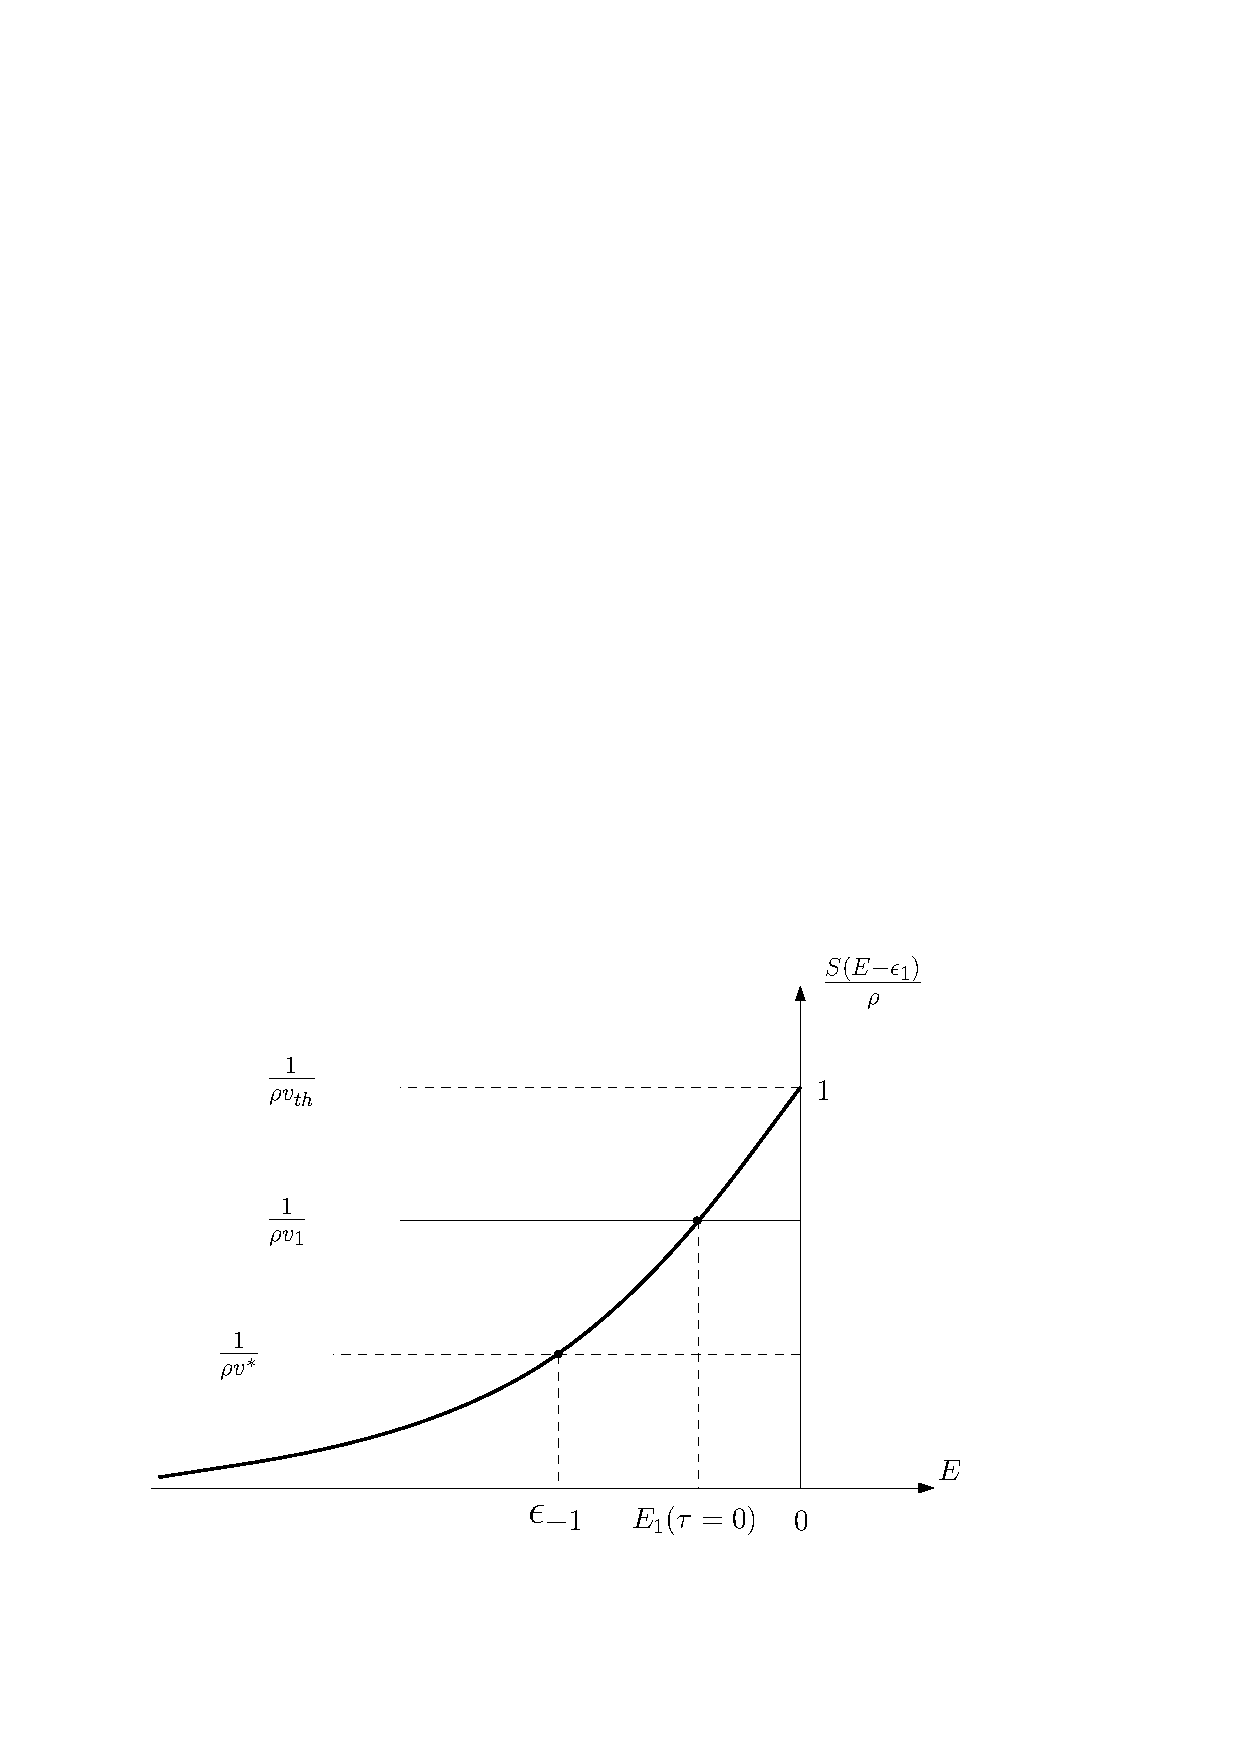
\includegraphics[width=.6\textwidth]{sDetail}
			\caption{Diagonal and non-diagonal subband interaction with shared species \label{fig:sDetail}}
\end{figure}
\subsubsection{With transfer $\tau$ but in the absence of potential within $(-1)$ subband, $v_{-1}=0$}
Eq.  \ref{eq:ssEq} for the one-pair energy follows from 
\begin{equation}
1-v_{1}S(E_1-\epsilon_{1})
=\tau^2S(E_1-\epsilon_{1})S(E_1-\epsilon_{-1})
\end{equation}
which also reads
\begin{equation}
S(E_1-\epsilon_{1})=\frac{1}{v_{1}+\tau^{2}S(E-\epsilon_{-1})}
\end{equation}
${v_{1}+\tau^{2}S(E-\epsilon_{-1})}$ can be seen as the potential of the subband $1$ dressed by its coupling to subband $-1$.  Since $S(E-\epsilon_{-1})$ varies from $\rho$ to zero when $E$ decreases from $\epsilon_{-1}$, ${1}/{\rho{}[v_{1}+\tau^{2}S(E-\epsilon_{-1})]}$ varies from $1/\rho{}v_{1}$ to $1/(\rho{}v_{1}+\rho^{2}\tau^{2})$ (see Fig \ref{fig:1rhov}). It has to be compared to $S(E-\epsilon_{1})/\rho$ shown in Fig. \ref{fig:sDetail}.  these regimes can be distinguished.  
\begin{figure}[htb]
	\centering
	       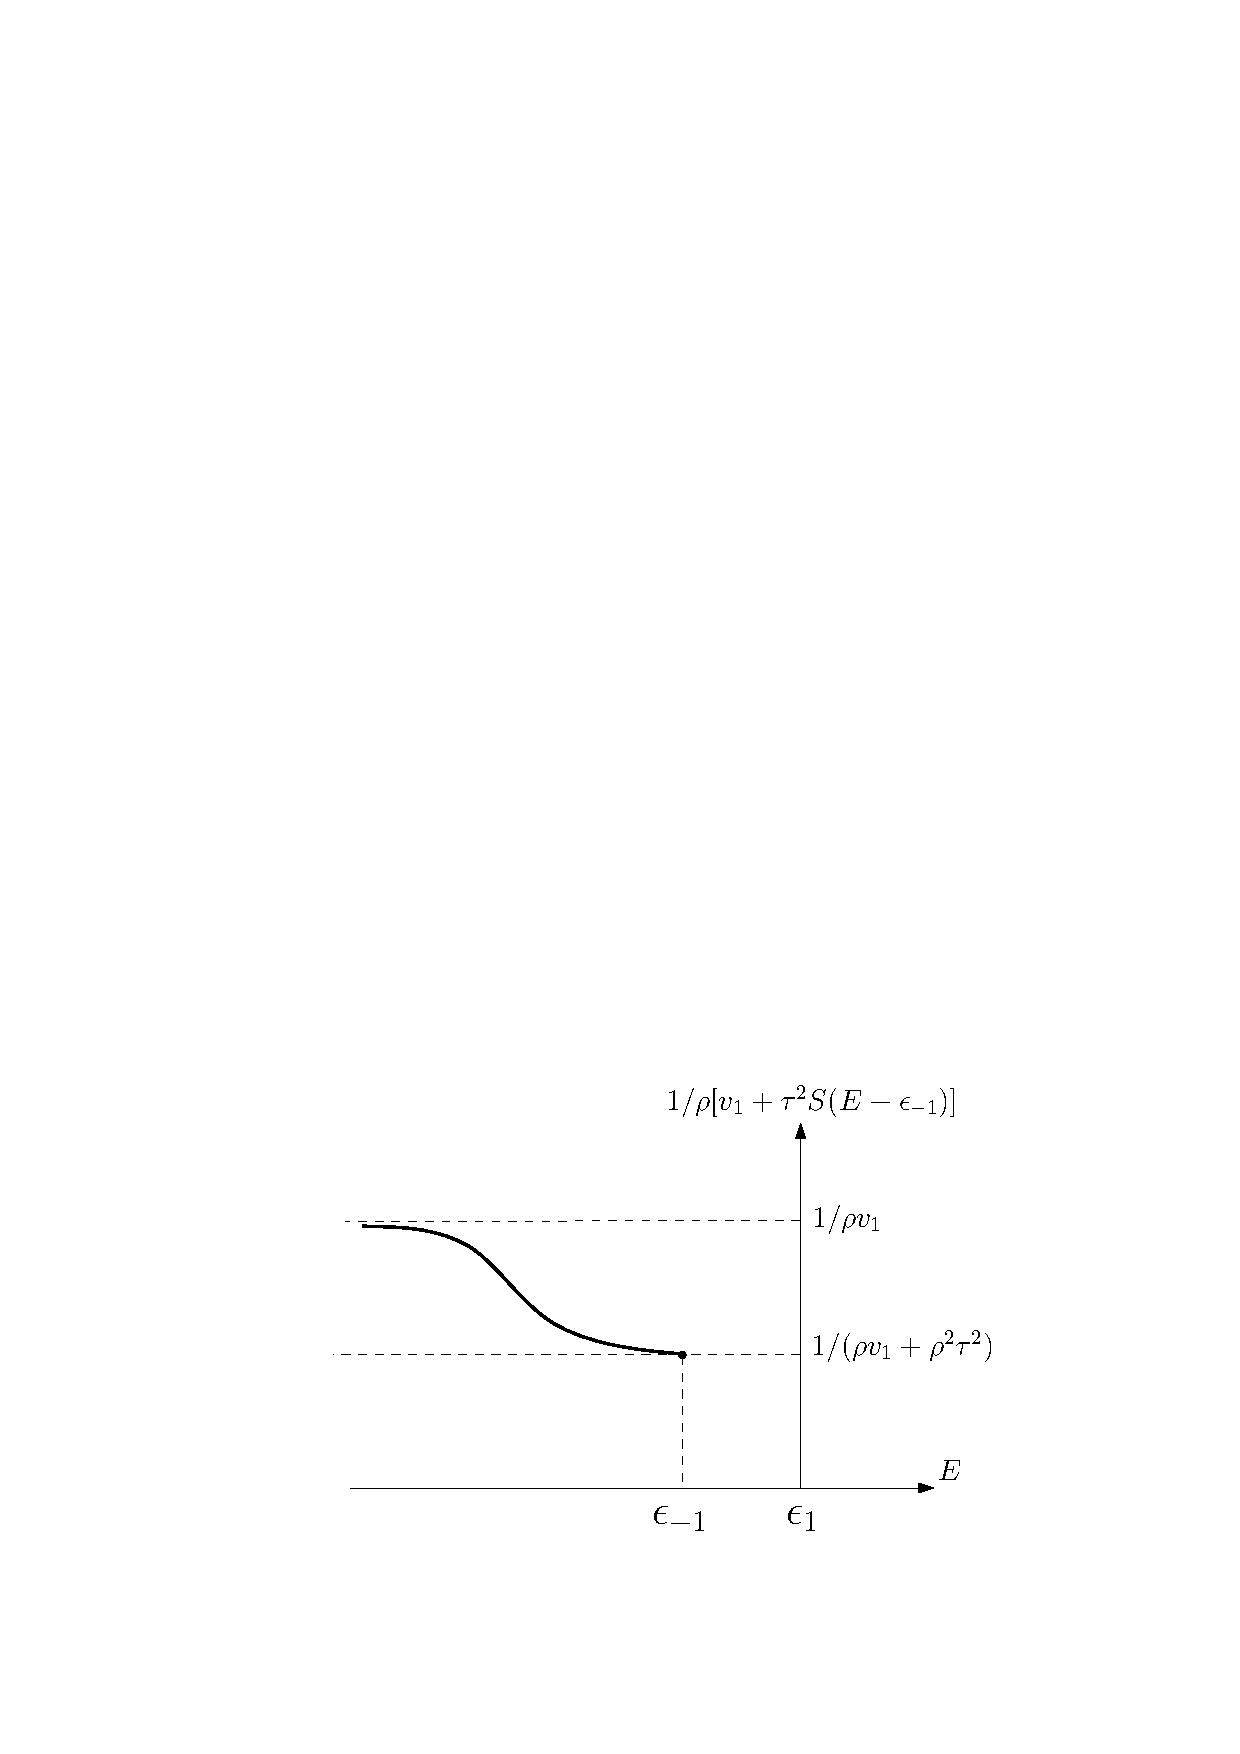
\includegraphics[width=.6\textwidth]{1rhov}
			\caption{Diagonal and non-diagonal subband interaction with shared species \label{fig:1rhov}}
\end{figure}

For $v_{\text{th}}$














\bibliography{../citation}
\bibliographystyle{plain}
\end{document}
